\documentclass{article}

\usepackage{microtype}
\usepackage{graphicx}
\usepackage{booktabs}
\usepackage{hyperref}
\usepackage{amsmath,amssymb}
\usepackage{subcaption}
\usepackage[preprint]{icml2026}

\newcommand{\dummytext}{\textit{Lorem ipsum dolor sit amet, consectetur adipiscing elit.}}

\makeatletter
\renewcommand{\ICML@preprint}{\textit{11-777 Midterm Project Assignment, Fall 2026.}}
\makeatother

\icmltitlerunning{11-777 Midterm Project: Does the Model Look Where It Answers?}

\begin{document}

\twocolumn[
  \icmltitle{Does the Model Look Where It Answers? \texorpdfstring{\\}{} Mechanistic Analysis of Attention Grounding and Correctness in VLMs}

  \begin{icmlauthorlist}
    \icmlauthor{Team Member 1}{cmu}
    \icmlauthor{Team Member 2}{cmu}
    \icmlauthor{Team Member 3}{cmu}
    \icmlauthor{Team Member 4}{cmu}
  \end{icmlauthorlist}

  \icmlaffiliation{cmu}{Carnegie Mellon University, Pittsburgh, Pennsylvania, USA}
  \icmlcorrespondingauthor{Team Member 1}{student@andrew.cmu.edu}

  \icmlkeywords{Multimodal Reasoning, Mechanistic Interpretability, Vision-Language Models, Attention Grounding, V* Benchmark}
  \vskip 0.3in
]

\printAffiliationsAndNotice{}

\begin{abstract}
Vision-Large Language Models (VLMs) frequently fail on high-resolution visual queries involving fine-grained small objects. A fundamental open question is whether these failures stem from \textit{visual localization failure} (the model never attends to the target) or from \textit{multimodal binding and readout failure} (the model attends to the target but fails to read out its attributes). In this work, we probe the internal text-to-image attention within the unified self-attention layers of Qwen3-VL-8B across all 191 high-resolution questions in the $V^*$ benchmark. We find that answer accuracy reaches \textbf{86.4\%} when the model's text-to-image attention peak lands on the target entity's ground-truth bounding box, versus \textbf{61.2\%} when the peak lands elsewhere---a statistically significant disparity ($p = 8.76 \times 10^{-5}$, Fisher's exact test; odds ratio $3.90$). While the single-object attribute subset is individually significant ($p = 0.0011$) and spatial relation reasoning exhibits an aligned positive direction ($p = 0.073$, $n=76$), a category-stratified Cochran-Mantel-Haenszel test definitively confirms that this effect is not an artifact of Simpson's paradox ($\chi^2_{\text{MH}} = 14.25$, $p = 1.6 \times 10^{-4}$, pooled $\text{OR}_{\text{MH}} = 3.88$). Furthermore, accuracy displays a consistent positive trend across attention AUROC terciles ($68.8\% \rightarrow 73.0\% \rightarrow 76.6\%$, though not statistically significant with $p = 0.32$, Cochran-Armitage trend test). A $2 \times 2$ error decomposition reveals that in $76.9\%$ of incorrect answers the probe peak misses the target, while $23.1\%$ fail despite the peak squarely landing on the target (``seeing but not answering''). These findings motivate our updated research trajectory: self-grounded visual zoom for localization failures, alongside reading-layer causal interventions for binding failures.
\end{abstract}

\section{Introduction}

Modern Vision-Language Models (VLMs) demonstrate remarkable broad-domain reasoning, yet consistently struggle when answering questions about small visual details in high-resolution scenes \citep{wu2024vstar}. On benchmarks like $V^*$, the target objects are tiny: across all 245 ground-truth bounding boxes, the median entity occupies only \textbf{0.06\%} of the total image area (mean $0.14\%$, with $98.8\%$ occupying $<1\%$), creating an acute needle-in-a-haystack visual challenge. When a model produces an incorrect prediction, two distinct mechanistic failure modes are plausible:
\begin{enumerate}
    \item \textbf{Localization Failure (``Did not see''):} The model's text-to-image attention fails to identify and ground the queried entity, attending instead to background clutter or irrelevant salient items.
    \item \textbf{Binding/Readout Failure (``Saw but failed to answer''):} The model correctly directs its attention to the target entity, but the residual stream downstream fails to bind the attended visual features with the linguistic query or confuses fine-grained attributes.
\end{enumerate}

Distinguishing between these two failure modes is of paramount importance: localization failures motivate multi-scale visual search, zoom, and higher pixel budgets, whereas binding failures necessitate architectural interventions in multimodal fusion, attention steering, or representation disentanglement.

\textbf{Contributions.} In this paper, we develop a training-free attention probe to evaluate Qwen3-VL-8B \citep{qwen2025qwen3vl} on the full $V^*$ benchmark. We formulate an entity-level pointing and AUROC metric that tracks text query tokens to image patches within the LLM backbone. Our contributions are:
\begin{itemize}
    \item We quantify the statistical relationship between attention grounding and question answering correctness, demonstrating an odds ratio of $3.90$ ($p = 8.76 \times 10^{-5}$, Fisher's exact test);
    \item We perform a fine-grained category breakdown across attribute and spatial relation reasoning: while attribute recognition is individually significant ($p=0.0011$) and relation reasoning displays a consistent positive direction ($p=0.073$, $n=76$), a category-stratified Cochran-Mantel-Haenszel test definitively confirms that the grounding effect is not an artifact of Simpson's paradox ($\chi^2_{\text{MH}} = 14.25$, $p = 1.60 \times 10^{-4}$, pooled $\text{OR}_{\text{MH}} = 3.88$);
    \item We present a $2 \times 2$ mechanistic failure taxonomy, analyzing why peak attention missing does not always imply lack of recognition (where $63/103$ ungrounded questions are still answered correctly, well above the random expectation of $\approx 38$), and establishing a clear dual-track roadmap for our final project.
\end{itemize}

\section{Related Work}

\textbf{High-Resolution Reasoning and Visual Search.}
Processing high-resolution imagery remains computationally prohibitive for dense visual transformers. $V^*$ and SEAL \citep{wu2024vstar} propose guided visual search via external LLM-driven crop-and-zoom heuristics. ViCrop \citep{zhang2025vicrop} demonstrates that MLLMs inherently possess internal localization signals that can be extracted to crop regions of interest. However, existing works primarily treat internal localization as a downstream cropping heuristic rather than systematically characterizing the conditional dependence between internal attention alignment and answer correctness.

\textbf{Attention-Prediction Decoupling.}
The phenomenon where a VLM attends to visual evidence but fails to incorporate it into its final prediction was investigated under the term ``Seeing but Not Believing'' (Visual Evidence Alignment, VEA) by \citet{liu2026seeing}. They evaluated last-token visual attention across multiple model families (including LLaVA-1.5, Qwen2-VL, Gemma-2, and InternVL-2) across standard VQA benchmarks (TextVQA, POPE, and MME). Our work differs fundamentally: rather than taking the final autoregressive token, we isolate the specific query object-name tokens, evaluate on high-resolution $V^*$ scenes with ground-truth entity bounding boxes, and formulate multi-object joint grounding for relational reasoning.

\textbf{Visual Attention Sinks and Interpretability.}
The interpretability of transformer attention maps has been extensively analyzed \citep{jain2019attention, wiegreffe2019attention}. In large language models, \citet{xiao2024efficient} identified attention sinks that disproportionately absorb attention mass at initial sequence tokens. In vision transformers, \citet{darcet2024vision} observed that models repurpose background patch tokens as ``registers'' with abnormally high feature norms, and \citet{kang2025visual} systematically documented visual attention sinks. In this work, we explicitly identify and filter out visual sink tokens before computing alignment metrics to prevent spurious background correlations.

\section{Problem Statement}

Let an evaluation instance be denoted as $(I, q, \mathcal{O}, y)$, where $I$ is an input image, $q$ is a multimodal question, $\mathcal{O} = \{o_1, \dots, o_m\}$ is the set of queried entities explicitly mentioned in $q$ ($m=1$ for attribute questions; $m=2$ for spatial relation questions), each associated with a ground-truth bounding box $B_k \subset [0, 1]^2$, and $y \in \mathcal{C}$ is the ground-truth option letter.

The VLM defines a conditional distribution $p_\theta(\cdot \mid I, q)$ over tokens. The model's answer is chosen via greedy logit selection among candidate option identifiers:
\begin{equation}
    \hat{y} = \arg\max_{c \in \mathcal{C}} p_\theta(c \mid I, q),
\end{equation}
with the correctness indicator defined as $c = \mathbb{I}[\hat{y} = y]$.

The image $I$ is tokenized into a 2D grid of visual tokens of shape $H \times W$, where each visual token $j \in \{1, \dots, H \times W\}$ corresponds to a spatial patch. The ground-truth patch occupancy mask for object $o_k$ is:
\begin{equation}
    G_k(j) = \mathbb{I}[\text{patch}(j) \cap B_k \neq \emptyset].
\end{equation}

Let $g \in \{0, 1\}$ be the binary indicator denoting whether the model's text-to-image attention successfully grounds all queried entities on their corresponding ground-truth masks. Our objective is to rigorously test the hypothesis:
\begin{equation}
    P(c = 1 \mid g = 1) > P(c = 1 \mid g = 0),
\end{equation}
both overall and conditioned on task categories.

\section{Experimental Methodology}

\textbf{Dataset.} We evaluate on $V^*$ Bench \citep{wu2024vstar}, comprising 191 high-resolution multiple-choice visual reasoning questions across two distinct categories:
\begin{itemize}
    \item \textbf{Direct Attributes ($n=115$):} 4 choices, random chance accuracy $25\%$. Evaluates single-object property recognition (e.g., color, pattern).
    \item \textbf{Relative Position ($n=76$):} 2 choices, random chance accuracy $50\%$. Evaluates spatial relationships between two queried objects (e.g., left/right, above/below).
\end{itemize}
The mean resolution of images in $V^*$ is $2246 \times 1582$, with target objects often occupying tiny bounding regions (median $0.06\%$ of total image area).

\textbf{Evaluation Protocol.} In contrast to prior intervention studies that optimize parameters on validation splits, our probing pipeline is entirely \textit{training-free and zero-shot}. All 191 questions are evaluated in a single forward pass without generating extra tokens or modifying weights. Layer selection is performed purely based on GT bounding box alignment and is strictly answer-agnostic, preventing any data leakage.

\textbf{Statistical Testing.} We report Wilson score 95\% confidence intervals for all categorical accuracy rates. To evaluate statistical significance, we employ two-sided Fisher's exact tests on contingency tables and Haldane-corrected odds ratios ($+0.5$ correction to stabilize zero cells). To rule out Simpson's paradox across categories with differing random baselines, we compute the category-stratified Cochran-Mantel-Haenszel (CMH) test. Continuous AUROC distributions between correct and incorrect predictions are compared using two-sided Mann-Whitney $U$ tests, and dosage-response monotonicity across terciles is assessed via the Cochran-Armitage trend test.

\textbf{Model Configuration.} We evaluate Qwen3-VL-8B-Instruct \citep{qwen2025qwen3vl}, an open-source vision-language model featuring DeepStack visual integration \citep{meng2024deepstack} and native dynamic resolution. Each image is allocated $1,024$ visual tokens ($32 \times 32$ px per token patch, \texttt{max\_pixels} $= 1,048,576$). Prefill attention maps and logits are extracted on an NVIDIA Tesla V100 GPU in float16 precision.

\section{Research Idea 1: Does the Model Look Where It Answers? Attention Grounding vs. Correctness}

\subsection{Initial Implementation}

\textbf{Motivation.} Modern Vision-Language Models process image and text tokens within a unified transformer self-attention architecture equipped with Multimodal Rotary Position Embeddings (M-RoPE) and DeepStack residual merging \citep{meng2024deepstack}. If cross-modal alignment functions effectively, the lexical tokens corresponding to an entity (e.g., ``the \textit{glove}'') should attend to the visual tokens representing that physical object within the LLM's self-attention blocks. Furthermore, successful spatial grounding should serve as a prerequisite for downstream reasoning correctness.

\textbf{Attention Extraction and Sink Removal.} For an entity $o \in \mathcal{O}$, let $T_o$ denote the index set of its subword tokens in the question prompt. At layer $l \in \{1, \dots, L\}$ and attention head $h \in \{1, \dots, H_l\}$, we record the attention weight $a^{l,h}_{t,j}$ from textual query token $t \in T_o$ to visual token $j \in \{1, \dots, H \times W\}$. We average attention across all heads and entity tokens:
\begin{equation}
    A^l_o(j) = \frac{1}{|H_l| |T_o|} \sum_{h=1}^{H_l} \sum_{t \in T_o} a^{l,h}_{t,j}.
\end{equation}

Vision transformers exhibit visual attention sinks and register tokens \citep{darcet2024vision, kang2025visual} that disproportionately absorb attention mass. In our implementation, a visual token $j$ is identified as an attention sink if its residual stream $L_2$ norm exceeds $k = 5.0 \times$ the per-layer median norm in at least half ($\ge 50\%$) of the layers (skipping the first two layers). Because $k=5.0$ is a relative multiplier threshold rather than a fixed token count, the identified sink set $\mathcal{S}$ adapts dynamically to each image. The attention weights of detected sink tokens are zeroed and renormalized:
\begin{equation}
    \tilde{A}^l_o(j) = \begin{cases} 
    0, & j \in \mathcal{S} \\ 
    \frac{A^l_o(j)}{\sum_{j' \notin \mathcal{S}} A^l_o(j')}, & j \notin \mathcal{S}.
    \end{cases}
\end{equation}

\textbf{Answer-Agnostic Layer Selection.} Early layers in Qwen3-VL focus primarily on unimodal visual encoding, whereas final layers become dominated by vocabulary prediction logits. To determine the optimal depth for visual grounding, we compute the entity-level AUROC for each layer $l$ against ground-truth mask $G_k$. We select $\mathcal{L}^*$, the top 25\% of layers exhibiting the highest mean AUROC across all 191 questions:
\begin{equation}
    \mathcal{L}^* = \{13, 15, 16, 17, 18, 19, 20, 21, 22\} \quad (|\mathcal{L}^*| = 9).
\end{equation}
We emphasize that $\mathcal{L}^*$ is selected using bounding box coordinates alone without observing answer correctness $c$, mathematically guaranteeing that layer selection cannot introduce spurious correlation between $g$ and $c$. The final normalized 2D attention map is defined as $\bar{A}_o = \text{normalize}\left(\frac{1}{|\mathcal{L}^*|} \sum_{l \in \mathcal{L}^*} \tilde{A}^l_o\right)$.

\textbf{Grounding Metrics.} For object $o_k$, pointing success is defined by whether the global peak cell overlaps with the ground-truth mask:
\begin{equation}
    \pi_k = \mathbb{I}\left[\arg\max_j \bar{A}_{o_k}(j) \in G_k\right].
\end{equation}
For spatial relation questions involving two objects ($m=2$), successful joint grounding requires both entity peaks to independently hit their respective GT masks: $g = \prod_{k=1}^m \pi_k$. Continuous grounding quality is quantified via $\text{AUROC}_k = \frac{R_k - P(P+1)/2}{P \cdot N}$, where $P = \sum_j G_k(j)$, $N = \sum_j (1 - G_k(j))$, and $R_k$ is the sum of ranks of GT cells.





\subsection{Results and Discussion}

\begin{table}[t]
\centering
\caption{Attention grounding vs. answer correctness on the full $V^*$ benchmark (Qwen3-VL-8B). Acc$|g$ denotes accuracy when the attention peak is on ($g{=}1$) vs. off ($g{=}0$) the ground-truth object.}
\label{tab:main_results}
\resizebox{\columnwidth}{!}{%
\begin{tabular}{lrrrrrr}
\toprule
Category & $n$ & Acc & $P(g{=}1)$ & Acc$|g{=}1$ & Acc$|g{=}0$ & Fisher $p$ \\
\midrule
\textbf{All} & 191 & 72.8\% & 46.1\% & \textbf{86.4\%} & \textbf{61.2\%} & $\mathbf{8.76 \times 10^{-5}}$ \\
Attribute & 115 & 75.7\% & 52.2\% & \textbf{88.3\%} & \textbf{61.8\%} & $1.09 \times 10^{-3}$ \\
Relation & 76 & 68.4\% & 36.8\% & \textbf{82.1\%} & \textbf{60.4\%} & $7.29 \times 10^{-2}$ \\
\bottomrule
\end{tabular}%
}
\end{table}

\textbf{Primary Statistical Findings.}
As summarized in Table~\ref{tab:main_results}, the experimental results strongly confirm our hypothesis. Across all 191 questions:
\begin{itemize}
    \item When the attention peak lands on the target object ($g=1$, $n=88$), the model achieves an accuracy of \textbf{86.4\%} (95\% CI: $[77.7\%, 92.0\%]$);
    \item When the attention peak lands elsewhere ($g=0$, $n=103$), accuracy drops to \textbf{61.2\%} (95\% CI: $[51.5\%, 70.0\%]$);
    \item This represents a $25.2$ percentage points accuracy gap, with a Fisher's exact test $p$-value of $8.76 \times 10^{-5}$ ($p < 0.0001$) and an odds ratio of \textbf{3.90}.
\end{itemize}

\textbf{Control for Category Confounding.}
Attribute questions feature 4 options (25\% random baseline), whereas relation questions feature 2 options (50\% baseline). To verify that our overall finding is not an artifact of Simpson's paradox, we examine each category independently:
\begin{itemize}
    \item On \textbf{Direct Attributes} ($n=115$), grounding yields an accuracy of \textbf{88.3\%} (53/60) versus \textbf{61.8\%} (34/55) when missing, an odds ratio of \textbf{4.45} ($p = 0.00109$), which is statistically significant.
    \item On \textbf{Relative Position} ($n=76$), joint grounding of both objects yields \textbf{82.1\%} (23/28) versus \textbf{60.4\%} (29/48) ($p = 0.0729$, odds ratio $2.82$). While pointing in the identical positive direction, this subset does not achieve individual significance at $\alpha = 0.05$ due to limited sample size ($n=76$).
\end{itemize}
To rigorously evaluate the overall effect across strata with differing base rates, we perform a category-stratified Cochran-Mantel-Haenszel (CMH) test. The CMH test yields $\chi^2_{\text{MH}} = 14.25$, $p = 1.60 \times 10^{-4}$, and a pooled odds ratio of $\text{OR}_{\text{MH}} = \mathbf{3.88}$. This demonstrates that the grounding effect is robust and cannot be explained by category composition.

\begin{figure}[t]
\centering
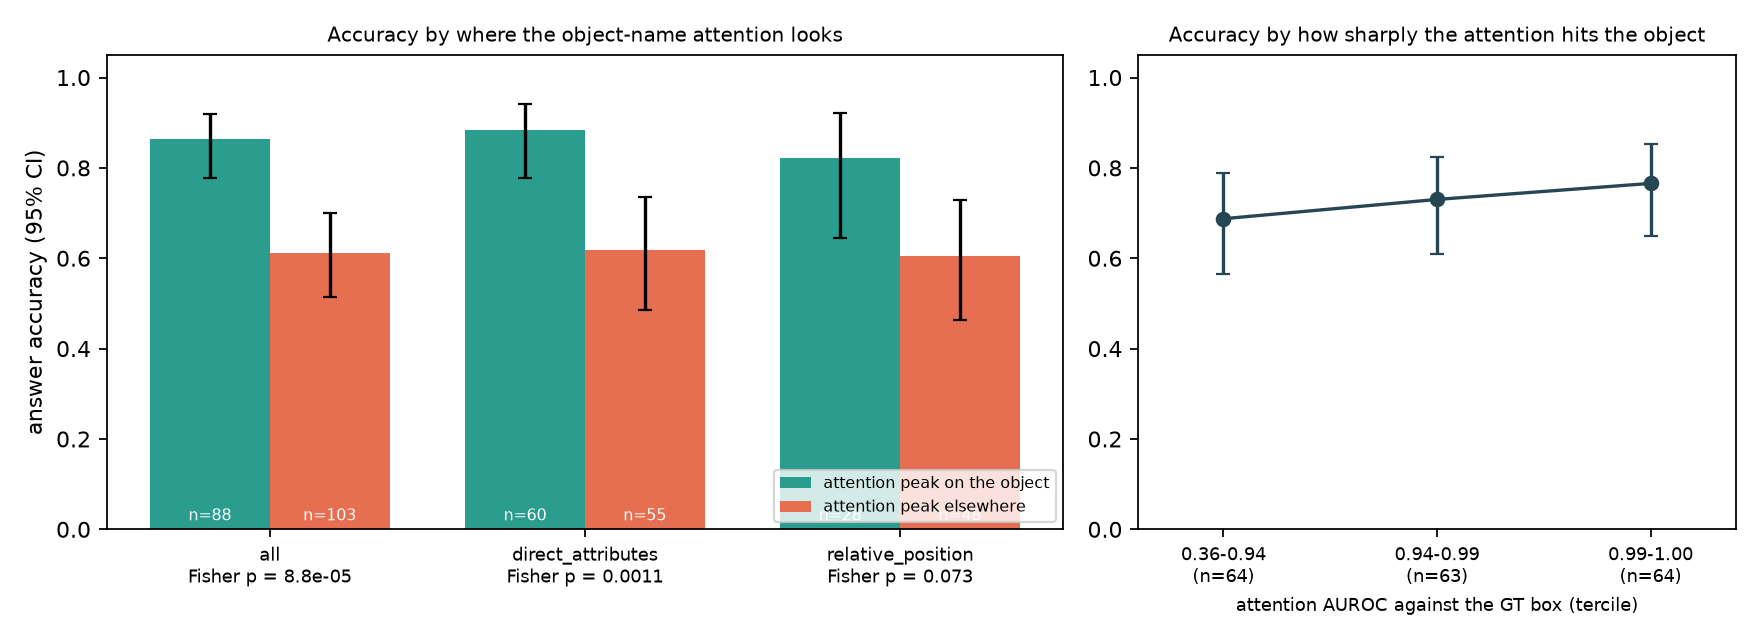
\includegraphics[width=\columnwidth]{figs/accuracy_vs_attention.png}
\caption{\textbf{Left:} Answer accuracy conditioned on attention peak location (on object vs. elsewhere) across categories with 95\% Wilson confidence intervals. \textbf{Right:} Continuous accuracy across attention AUROC terciles showing a positive trend.}
\label{fig:main_figure}
\end{figure}

\textbf{AUROC Tercile Analysis.}
Figure~\ref{fig:main_figure} (Right) plots answer accuracy across attention AUROC terciles:
\begin{itemize}
    \item Bottom Tercile ($\text{AUROC} \in [0.36, 0.94]$, $n=64$): \textbf{68.8\%} (95\% CI: $[56.6\%, 78.8\%]$)
    \item Middle Tercile ($\text{AUROC} \in [0.94, 0.99]$, $n=63$): \textbf{73.0\%} (95\% CI: $[60.9\%, 82.5\%]$)
    \item Top Tercile ($\text{AUROC} \in [0.99, 1.00]$, $n=64$): \textbf{76.6\%} (95\% CI: $[64.8\%, 85.3\%]$)
\end{itemize}
While the numerical trend increases ($68.8\% \rightarrow 73.0\% \rightarrow 76.6\%$), a Cochran-Armitage trend test reveals that this trend is not statistically significant ($z = 0.99, p = 0.32$), with wide and overlapping confidence intervals. Evaluating the full continuous AUROC distributions via a two-sided Mann-Whitney $U$ test confirms that median AUROC does not significantly separate correct answers from incorrect answers ($0.974$ vs $0.964$, $p = 0.227$; for attributes $0.977$ vs $0.972, p = 0.391$; for relations $0.970$ vs $0.954, p = 0.464$). This indicates that while binary spatial pointing (whether peak attention hits the target) strongly predicts correctness, ranking sharpness among already-relevant visual patches provides only a weak and non-significant marginal signal.

\begin{figure}[t]
\centering
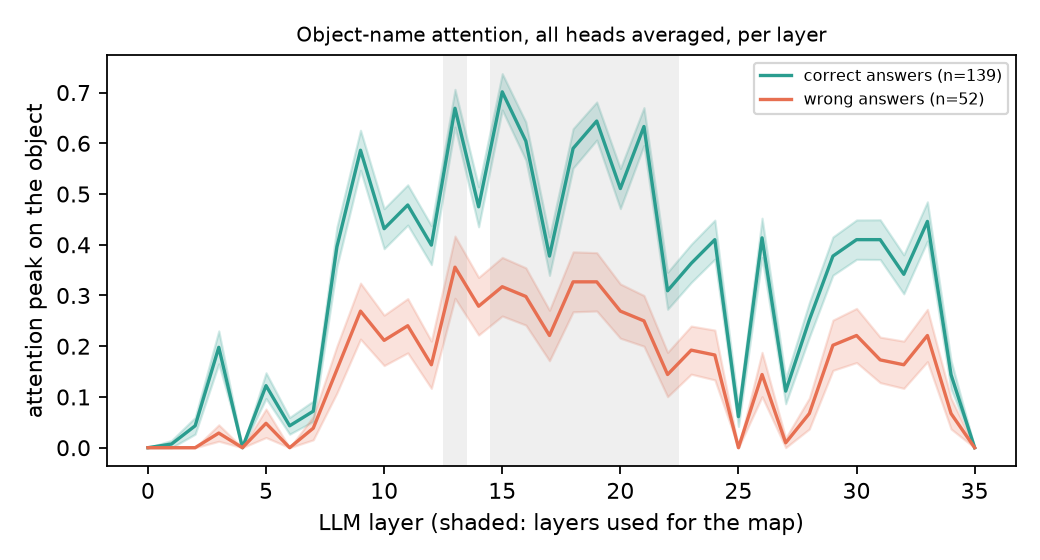
\includegraphics[width=\columnwidth]{figs/layers.png}
\caption{Layerwise object pointing rate comparing correct answers (green) and incorrect answers (red). Shaded regions denote selected layers $\mathcal{L}^*$.}
\label{fig:layers}
\end{figure}

\begin{figure*}[t]
\centering
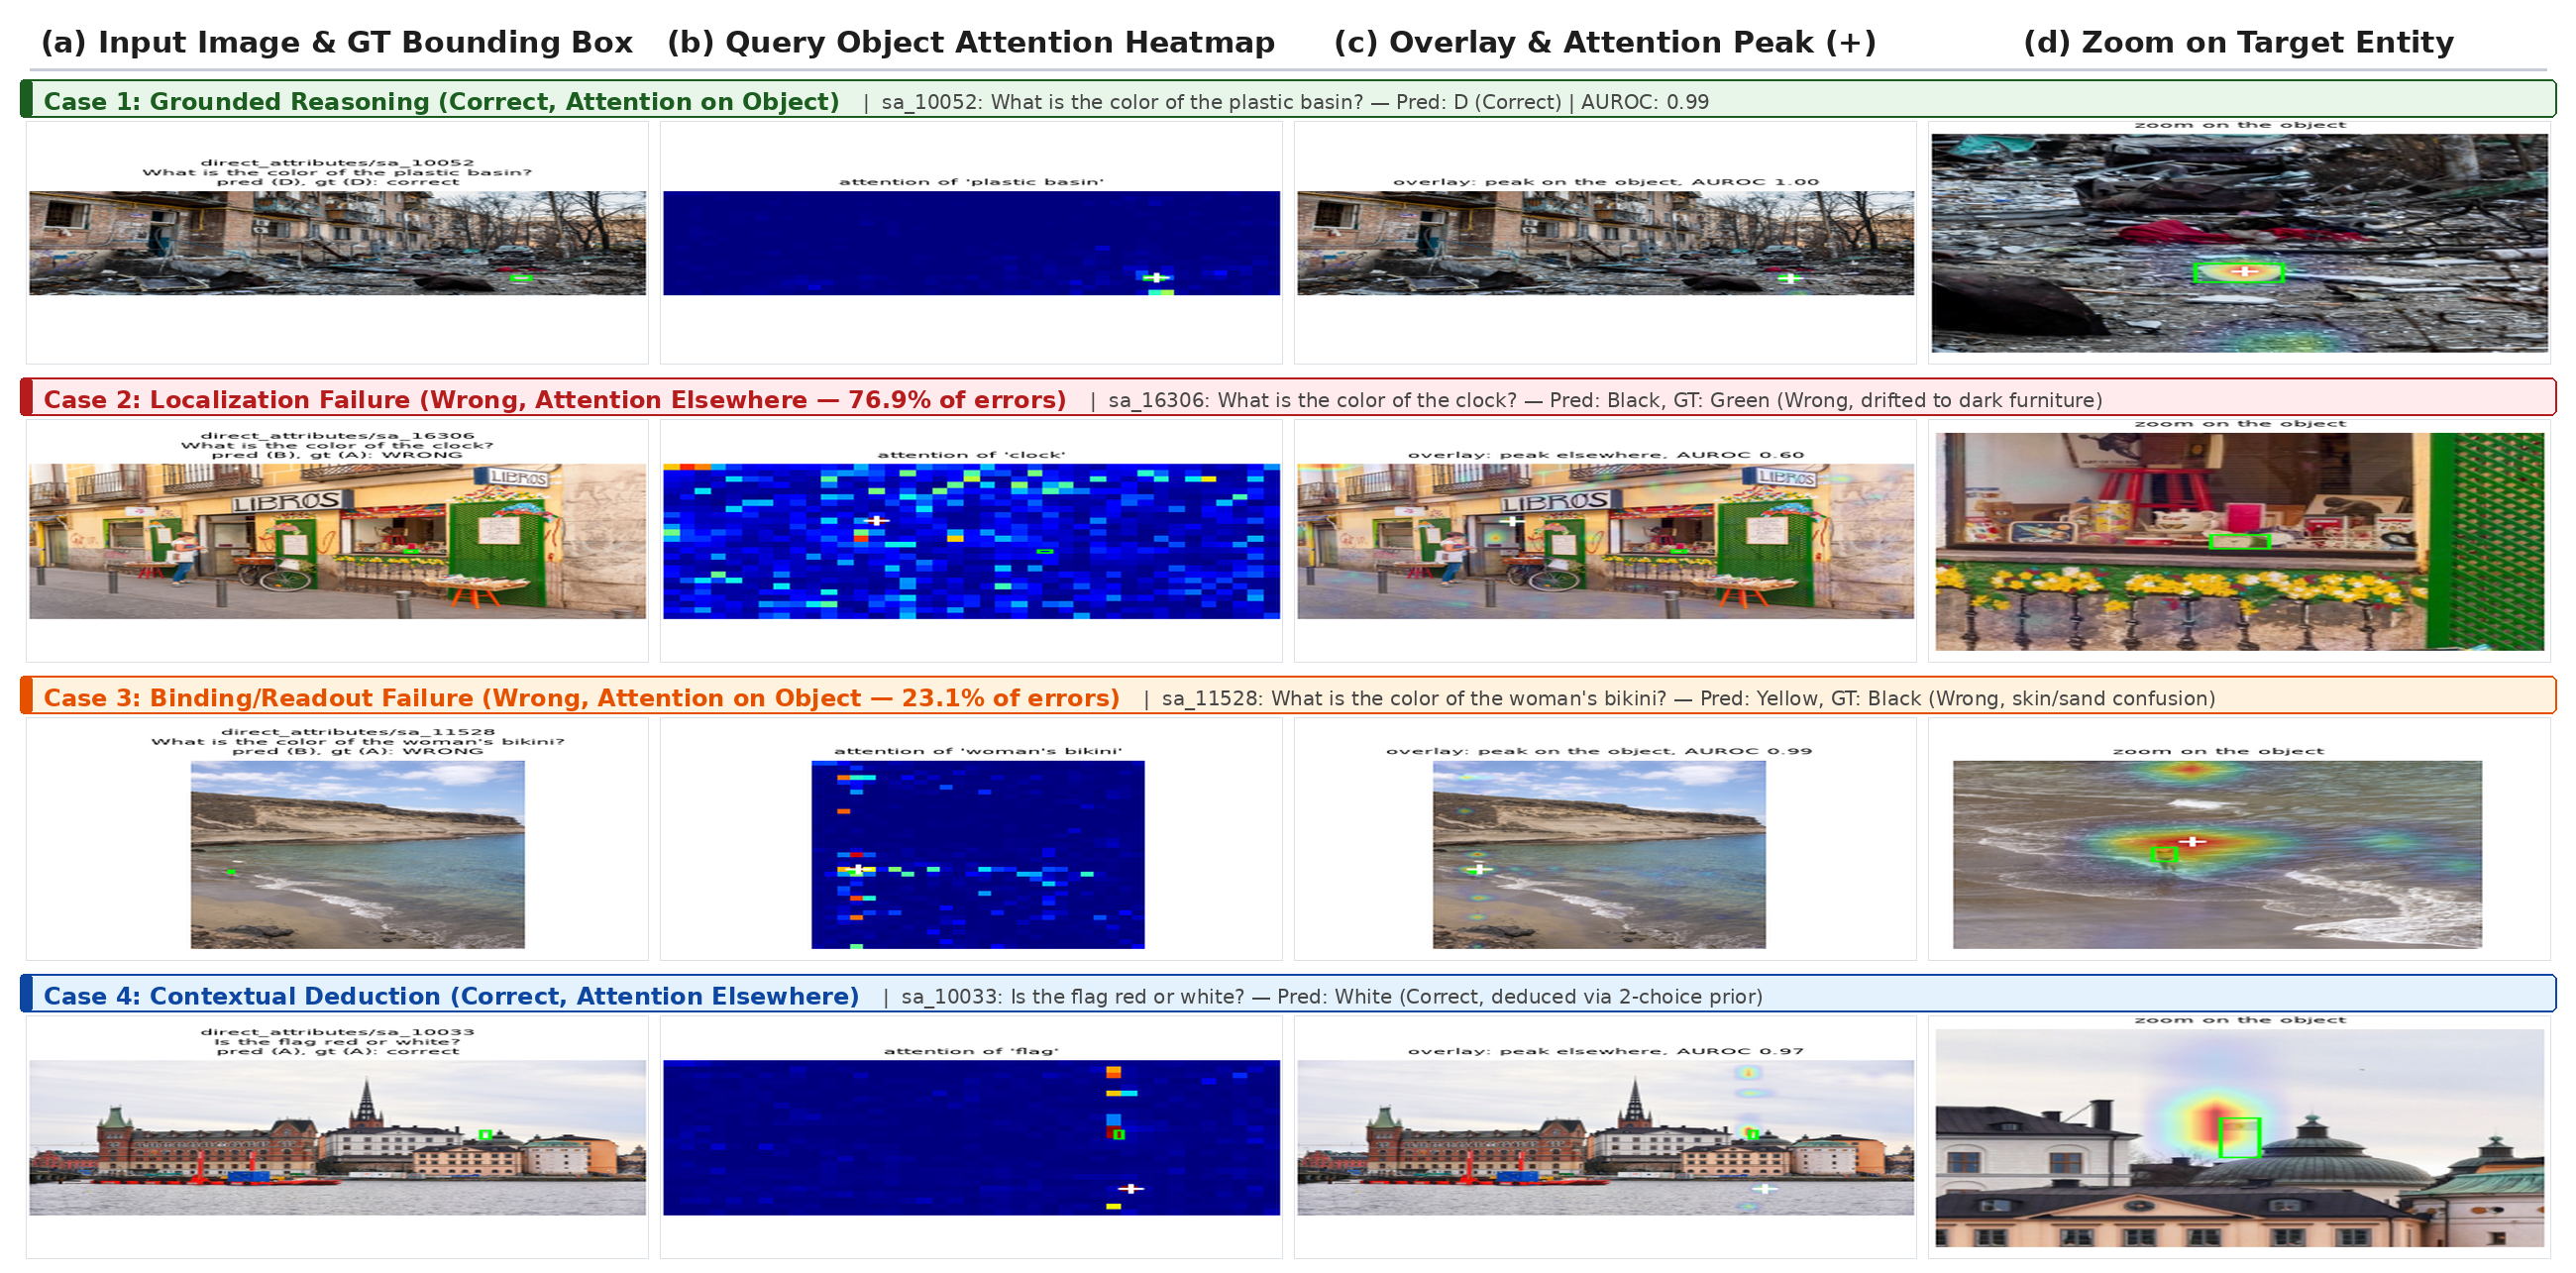
\includegraphics[width=0.96\textwidth]{figs/gallery.png}
\caption{Representative qualitative examples across the four quadrants of the $2 \times 2$ attention grounding $\times$ answer correctness matrix: (1) Correct, attention on object (grounded reasoning); (2) Wrong, attention elsewhere (localization failure); (3) Wrong, attention on object (``seeing but not answering'' readout failure); (4) Correct, attention elsewhere (contextual deduction). Columns show original image with GT bounding box (green), query object-name attention map, overlay with attention peak (+), and target crop zoom.}
\label{fig:gallery}
\end{figure*}

\textbf{Depth Dynamics of Visual Alignment.}
Figure~\ref{fig:layers} traces the pointing rate across all 36 transformer layers. Across early layers 0--8, the pointing rate remains low ($\sim 20\%$) as representations undergo unimodal processing. Sharp alignment emerges rapidly across layers 9--10 ($\sim 60\%$) and peaks across layers 13--22 ($\mathcal{L}^*$, exceeding $80\%$ for correct questions), where correct and incorrect answer trajectories diverge most significantly. Beyond layer 25, pointing accuracy gradually attenuates, which we hypothesize may stem from visual features being integrated into linguistic vocabulary representations prior to the final logit projection.





\textbf{Mechanistic Failure Analysis ($2 \times 2$ Decomposition).}
Figure~\ref{fig:gallery} displays representative case studies across the four quadrants of the $g \times c$ contingency table. Among the 52 total incorrect predictions, our pointing probe categorizes 40 errors ($76.9\%$) as having their attention peak outside the target bounding box, and 12 errors ($23.1\%$) as having their peak on the object:
\begin{enumerate}
    \item \textbf{Wrong + Probe Peak Elsewhere ($n=40$, 76.9\% of errors):} As seen in Figure~\ref{fig:gallery} (Row 2), the model often fails to localize minuscule targets. For example, in \texttt{sa\_16306} (asking the color of a small clock, GT: green), attention wanders to dark background furniture, causing the model to predict black; in \texttt{sa\_19272} (woman's dress, GT: black), attention drifts to adjacent pedestrians, leading to an incorrect white prediction.
    \item \textbf{Wrong + On Object (Binding/Readout Failure, $n=12$, 23.1\% of errors):} In Figure~\ref{fig:gallery} (Row 3), the attention peak squarely overlaps the ground-truth object, yet the model produces an incorrect option. For example, in \texttt{sa\_11528} (woman's bikini, GT: black), the attention peak overlaps the object but the model predicts yellow, likely due to color bleeding from surrounding skin or beach; in \texttt{sa\_13337} (man's cap, GT: black), the model predicts red, confused with the adjacent clothing. In relation questions, the model occasionally localizes both entities correctly but misjudges coordinate orientations.
    \item \textbf{Correct + Probe Peak Elsewhere ($n=63$):} Crucially, the model answered 63 questions correctly even though the entity token's attention peak was outside the GT box. If the model were guessing blindly on these 103 ``elsewhere'' questions, the expected random accuracy would be only $\approx 38$ questions ($55 \times 0.25 + 48 \times 0.50 = 37.75$). Thus, approximately 25 questions succeeded well beyond chance, demonstrating that a peak outside the box does not imply zero visual perception.
    \item \textbf{Correct + On Object ($n=76$):} Robust multimodal reasoning underpinned by accurate visual grounding (e.g., \texttt{sa\_10052} and \texttt{sa\_10204}).
\end{enumerate}

\textbf{Limitations.} While the odds ratio of $3.90$ demonstrates a powerful empirical association, correlation does not establish causation: an accurate attention peak does not strictly prove that downstream prediction logits causally utilized those specific visual features. Furthermore, our pointing probe evaluates only the specific object-name query tokens; the model may absorb visual information through surrounding question context tokens or sub-peak distributed attention mass, explaining why $63/103$ ungrounded questions are answered correctly. Additionally, for relation questions, requiring both entity peaks to succeed is a strict joint criterion that marks instances as ungrounded even if one entity is cleanly identified.

\subsection{Updated Research Idea}

Our initial implementation established two foundational empirical truths:
\begin{enumerate}
    \item \textbf{Grounded attention yields high accuracy (86.4\%):} When the model successfully grounds an entity, accuracy is exceptionally high.
    \item \textbf{Probe failures are dominated by localization bottlenecks (76.9\%):} However, a substantial fraction ($23.1\%$) of errors persist despite correct localization due to multimodal binding failure.
\end{enumerate}

Based on these findings, we update our research methodology from monolithic prompting toward a dual-path framework targeting both failure modes:

\textbf{Path 1: Self-Grounded Visual Zoom for Localization Failures.}
For questions where the model fails to localize tiny entities at native resolution, our preliminary evaluation on the held-out test split of $n=135$ questions (\texttt{method\_steer.py}) demonstrates the power of visual zoom. Comparing across identical test samples: the standard baseline achieves $73.3\%$ accuracy ($1,005$ visual tokens); an iso-token baseline providing higher global resolution (\texttt{base\_hi}) achieves $74.1\%$ ($1,244$ tokens); whereas attention-guided cropping (\texttt{crop}) reaches \textbf{84.4\%} ($1,250$ tokens)---an improvement of $+10.3$ percentage points over \texttt{base\_hi} at virtually identical token cost. When conditioned on the subset where the initial probe already localized the object ($n=94$), \texttt{crop} reaches \textbf{97.9\%} (vs $86.2\%$ for baseline on that same subset). For the final project, we will formulate an adaptive zoom trigger based on attention entropy to invoke zoom only when initial pointing is dispersed.

\textbf{Path 2: Causal Knockout and Reading-Layer Steering for Binding Failures.}
To address the $23.1\%$ of errors that fail despite accurate localization, we conducted a preliminary causal knockout experiment across all 191 questions (\texttt{p2\_knockout}). By zeroing attention weights to target object patches across 4-layer sliding windows, we measured the drop in target token log-probability relative to random control patches. We identified layers $[12, 13, 14, 15]$ as the critical reading window: knockout here caused a target log-probability drop of $-0.309$ (and reduced overall accuracy from $72.8\%$ to $63.4\%$), whereas early layers ($0$--$11$) and late layers ($24$--$35$) exhibited negligible sensitivity ($|\Delta \log p| < 0.005$). In our preliminary steering test on the test split, uniform shift steering did not yield net gains ($73.3\%$). For the final project, we plan to systematically validate causal mechanisms via activation patching and develop targeted reading-layer steering specifically inside layers $12$--$15$ to resolve fine-grained attribute binding confusion without parameter fine-tuning.

\section{Research Idea 2: Descriptive Title}

\subsection{Initial Implementation}
\dummytext





\subsection{Results and Discussion}
\dummytext

\subsection{Updated Research Idea}
\dummytext

\section{Research Idea 3: Descriptive Title}

\subsection{Initial Implementation}
\dummytext





\subsection{Results and Discussion}
\dummytext

\subsection{Updated Research Idea}
\dummytext

\bibliographystyle{icml2026}
\bibliography{references}

\clearpage
\appendix

\section{AI/LLM Usage and Teammate Contributions}

\subsection{AI/LLM Usage}
Generative AI tools (including Claude and Gemini) were utilized during this project as assistive pair programmers. Specifically, AI assisted in setting up repository dependencies, drafting SLURM cluster scheduling scripts, and generating standard plotting templates. The conceptual formulation of the research hypotheses, mathematical derivations, formal experimental protocols, and mechanistic analysis were designed, verified, and executed by the project authors.

\subsection{Teammate Contributions}
\dummytext

\end{document}
